%%%%%%%%%%%%%%%%%%%%%%%%%%%%%%%%%%%%%%%%%
% Programming/Coding Assignment
% LaTeX Template
%
% This template has been downloaded from:
% http://www.latextemplates.com
%
% Original author:
% Ted Pavlic (http://www.tedpavlic.com)
%
% Note:
% The \lipsum[#] commands throughout this template generate dummy text
% to fill the template out. These commands should all be removed when 
% writing assignment content.
%
% This template uses a Perl script as an example snippet of code, most other
% languages are also usable. Configure them in the "CODE INCLUSION 
% CONFIGURATION" section.
%
%%%%%%%%%%%%%%%%%%%%%%%%%%%%%%%%%%%%%%%%%

%----------------------------------------------------------------------------------------
%	PACKAGES AND OTHER DOCUMENT CONFIGURATIONS
%----------------------------------------------------------------------------------------

\documentclass{article}
\usepackage{cite}

\usepackage{fancyhdr} % Required for custom headers
\usepackage{lastpage} % Required to determine the last page for the footer
\usepackage{extramarks} % Required for headers and footers
\usepackage[usenames,dvipsnames]{color} % Required for custom colors
\usepackage{graphicx} % Required to insert images
\usepackage{listings} % Required for insertion of code
\usepackage{courier} % Required for the courier font
\usepackage{lipsum} % Used for inserting dummy 'Lorem ipsum' text into the template
\usepackage{amsmath}
\usepackage{url}

% Margins
\topmargin=-0.45in
\evensidemargin=0in
\oddsidemargin=0in
\textwidth=6.5in
\textheight=9.0in
\headsep=0.25in

\linespread{1.1} % Line spacing

% Set up the header and footer
\pagestyle{fancy}
\lhead{\hmwkAuthorName} % Top left header
\chead{\hmwkClass\ (\hmwkClassInstructor\ \hmwkClassTime): \hmwkTitle} % Top center head
\rhead{\firstxmark} % Top right header
\lfoot{\lastxmark} % Bottom left footer
\cfoot{} % Bottom center footer
\rfoot{Page\ \thepage\ of\ \protect\pageref{LastPage}} % Bottom right footer
\renewcommand\headrulewidth{0.4pt} % Size of the header rule
\renewcommand\footrulewidth{0.4pt} % Size of the footer rule

\setlength\parindent{0pt} % Removes all indentation from paragraphs

%----------------------------------------------------------------------------------------
%	CODE INCLUSION CONFIGURATION
%----------------------------------------------------------------------------------------

\definecolor{MyDarkGreen}{rgb}{0.0,0.4,0.0} % This is the color used for comments
\lstloadlanguages{Perl} % Load Perl syntax for listings, for a list of other languages supported see: ftp://ftp.tex.ac.uk/tex-archive/macros/latex/contrib/listings/listings.pdf
\lstset{language=Perl, % Use Perl in this example
        frame=single, % Single frame around code
        basicstyle=\small\ttfamily, % Use small true type font
        keywordstyle=[1]\color{Blue}\bf, % Perl functions bold and blue
        keywordstyle=[2]\color{Purple}, % Perl function arguments purple
        keywordstyle=[3]\color{Blue}\underbar, % Custom functions underlined and blue
        identifierstyle=, % Nothing special about identifiers                                         
        commentstyle=\usefont{T1}{pcr}{m}{sl}\color{MyDarkGreen}\small, % Comments small dark green courier font
        stringstyle=\color{Purple}, % Strings are purple
        showstringspaces=false, % Don't put marks in string spaces
        tabsize=5, % 5 spaces per tab
        %
        % Put standard Perl functions not included in the default language here
        morekeywords={rand},
        %
        % Put Perl function parameters here
        morekeywords=[2]{on, off, interp},
        %
        % Put user defined functions here
        morekeywords=[3]{test},
       	%
        morecomment=[l][\color{Blue}]{...}, % Line continuation (...) like blue comment
        numbers=left, % Line numbers on left
        firstnumber=1, % Line numbers start with line 1
        numberstyle=\tiny\color{Blue}, % Line numbers are blue and small
        stepnumber=5 % Line numbers go in steps of 5
}

% Creates a new command to include a perl script, the first parameter is the filename of the script (without .pl), the second parameter is the caption
%\newcommand{\perlscript}[2]{
%\begin{itemize}
%\item[]\lstinputlisting[caption=#2,label=#1]{#1.pl}
%\end{itemize}
%}

%----------------------------------------------------------------------------------------
%	DOCUMENT STRUCTURE COMMANDS
%	Skip this unless you know what you're doing
%----------------------------------------------------------------------------------------

% Header and footer for when a page split occurs within a problem environment
\newcommand{\enterProblemHeader}[1]{
\nobreak\extramarks{#1}{#1 continued on next page\ldots}\nobreak
\nobreak\extramarks{#1 (continued)}{#1 continued on next page\ldots}\nobreak
}

% Header and footer for when a page split occurs between problem environments
\newcommand{\exitProblemHeader}[1]{
\nobreak\extramarks{#1 (continued)}{#1 continued on next page\ldots}\nobreak
\nobreak\extramarks{#1}{}\nobreak
}

\setcounter{secnumdepth}{0} % Removes default section numbers
\newcounter{homeworkProblemCounter} % Creates a counter to keep track of the number of problems

\newcommand{\homeworkProblemName}{}
\newenvironment{homeworkProblem}[1][Problem \arabic{homeworkProblemCounter}]{ % Makes a new environment called homeworkProblem which takes 1 argument (custom name) but the default is "Problem #"
\stepcounter{homeworkProblemCounter} % Increase counter for number of problems
\renewcommand{\homeworkProblemName}{#1} % Assign \homeworkProblemName the name of the problem
\section{\homeworkProblemName} % Make a section in the document with the custom problem count
\enterProblemHeader{\homeworkProblemName} % Header and footer within the environment
}{
\exitProblemHeader{\homeworkProblemName} % Header and footer after the environment
}

\newcommand{\problemAnswer}[1]{ % Defines the problem answer command with the content as the only argument
\noindent\framebox[\columnwidth][c]{\begin{minipage}{0.98\columnwidth}#1\end{minipage}} % Makes the box around the problem answer and puts the content inside
}

\newcommand{\homeworkSectionName}{}
\newenvironment{homeworkSection}[1]{ % New environment for sections within homework problems, takes 1 argument - the name of the section
\renewcommand{\homeworkSectionName}{#1} % Assign \homeworkSectionName to the name of the section from the environment argument
\subsection{\homeworkSectionName} % Make a subsection with the custom name of the subsection
\enterProblemHeader{\homeworkProblemName\ [\homeworkSectionName]} % Header and footer within the environment
}{
\enterProblemHeader{\homeworkProblemName} % Header and footer after the environment
}

%----------------------------------------------------------------------------------------
%	NAME AND CLASS SECTION
%----------------------------------------------------------------------------------------

\newcommand{\hmwkTitle}{Assignment\ \#9} % Assignment title
\newcommand{\hmwkDueDate}{Thursday,\ December 4,\ 2014} % Due date
\newcommand{\hmwkClass}{CS\ 595} % Course/class
\newcommand{\hmwkClassTime}{4:20pm} % Class/lecture time
\newcommand{\hmwkClassInstructor}{Dr. Nelson} % Teacher/lecturer
\newcommand{\hmwkAuthorName}{Holly Harkins} % Your name

%----------------------------------------------------------------------------------------
%	TITLE PAGE
%----------------------------------------------------------------------------------------

\title{
\vspace{2in}
\textmd{\textbf{\hmwkClass:\ \hmwkTitle}}\\
\normalsize\vspace{0.1in}\small{Due\ on\ \hmwkDueDate}\\
\vspace{0.1in}\large{\textit{\hmwkClassInstructor\ \hmwkClassTime}}
\vspace{3in}
}

\author{\textbf{\hmwkAuthorName}}
\date{} % Insert date here if you want it to appear below your name

%----------------------------------------------------------------------------------------

\begin{document}

\maketitle

%----------------------------------------------------------------------------------------
%	TABLE OF CONTENTS
%----------------------------------------------------------------------------------------

%\setcounter{tocdepth}{1} % Uncomment this line if you don't want subsections listed in the ToC

\newpage
\tableofcontents
\newpage

%----------------------------------------------------------------------------------------
%	PROBLEM 1
%----------------------------------------------------------------------------------------

% To have just one problem per page, simply put a \clearpage after each problem

\begin{homeworkProblem}
%Listing \ref{part1} shows a Perl script.
%\lipsum[1]

\begin{verbatim}

Create a blog-term matrix.  Start by grabbing 100 blogs; include:

http://f-measure.blogspot.com/
http://ws-dl.blogspot.com/

and grab 98 more as per the method shown in class.

Use the blog title as the identifier for each blog (and row of the
matrix).  Use the terms from every item/title (RSS) or entry/title
(Atom) for the columns of the matrix.  The values are the frequency
of occurrence.  Essentially you are replicating the format of the
"blogdata.txt" file included with the PCI book code.  Limit the
number of terms to the most "popular" (i.e., frequent) 500 terms,
this is *after* the criteria on p. 32 (slide 7) has been satisfied.

Create a histogram of how many pages each blog has (e.g., 30
blogs with just one page, 27 with two pages, 29 with 3 pages and 
so on).  

\end{verbatim}

%\lstinputlisting[breaklines=true, caption=Part1 Python]{convertJson.py}

\begin{verbatim}

Answer:

I used generateURLs.py to capture the 98 Blogs (feedlist.txt).  

Next step was to create a matrix. The matrix required was using blog title 
as the identifier for each blog row and using the terms for the columns of 
the matrix. The values are the frequency of occurrence. Using 
generatefeedvector.py, TFIDF is calculated as the score that balances the 
frequency of a term in a document vs. frequency of a term in all the 
documents.  A limit to the number of terms to the most "popular" 500 terms 
(blogdata.txt).

To create the Histogram, I used getNextPage.py to generate a count of how 
many pages each blog has (numberOfPages.txt).  Unfortunately I ran out of 
time and did not generate the count.  There was an error in the code I 
could not resolve.  I would have used R code to generate the histogram.


\end{verbatim}

\lstinputlisting[breaklines=true, caption=Generating Blog URLs]{generateUrls.py}
\lstinputlisting[breaklines=true, caption=Generating Matrix]{generatefeedvector.py}

%\perlscript{part1}{Sample Perl Script With Highlighting}

\clearpage

\end{homeworkProblem}
\clearpage

%----------------------------------------------------------------------------------------
%	PROBLEM 2
%----------------------------------------------------------------------------------------

\begin{homeworkProblem}
%Listing \ref{part2} shows a Perl script.
%\lipsum[2]

\begin{verbatim}

Create an ASCII and JPEG dendrogram that clusters (i.e., HAC)
the most similar blogs (see slides 12 & 13).  Include the JPEG in
your report and upload the ascii file to github (it will be too
unwieldy for inclusion in the report).

\end{verbatim}

\begin{verbatim}

Answer:

Assignment9.py uses Pearsons correlation and averages the data for the 2
old clusters.  The final cluster returned can be searched recursively to
recreate all the clusters and their end nodes (ASCII.txt).

The drawdendrogram function uses the Python Imaging Library to generate
Clust_Dendrogram.jpg.

Below is the dendogram that was created from the blog matrix.  

\end{verbatim}

\begin{figure}[!ht]
\centering
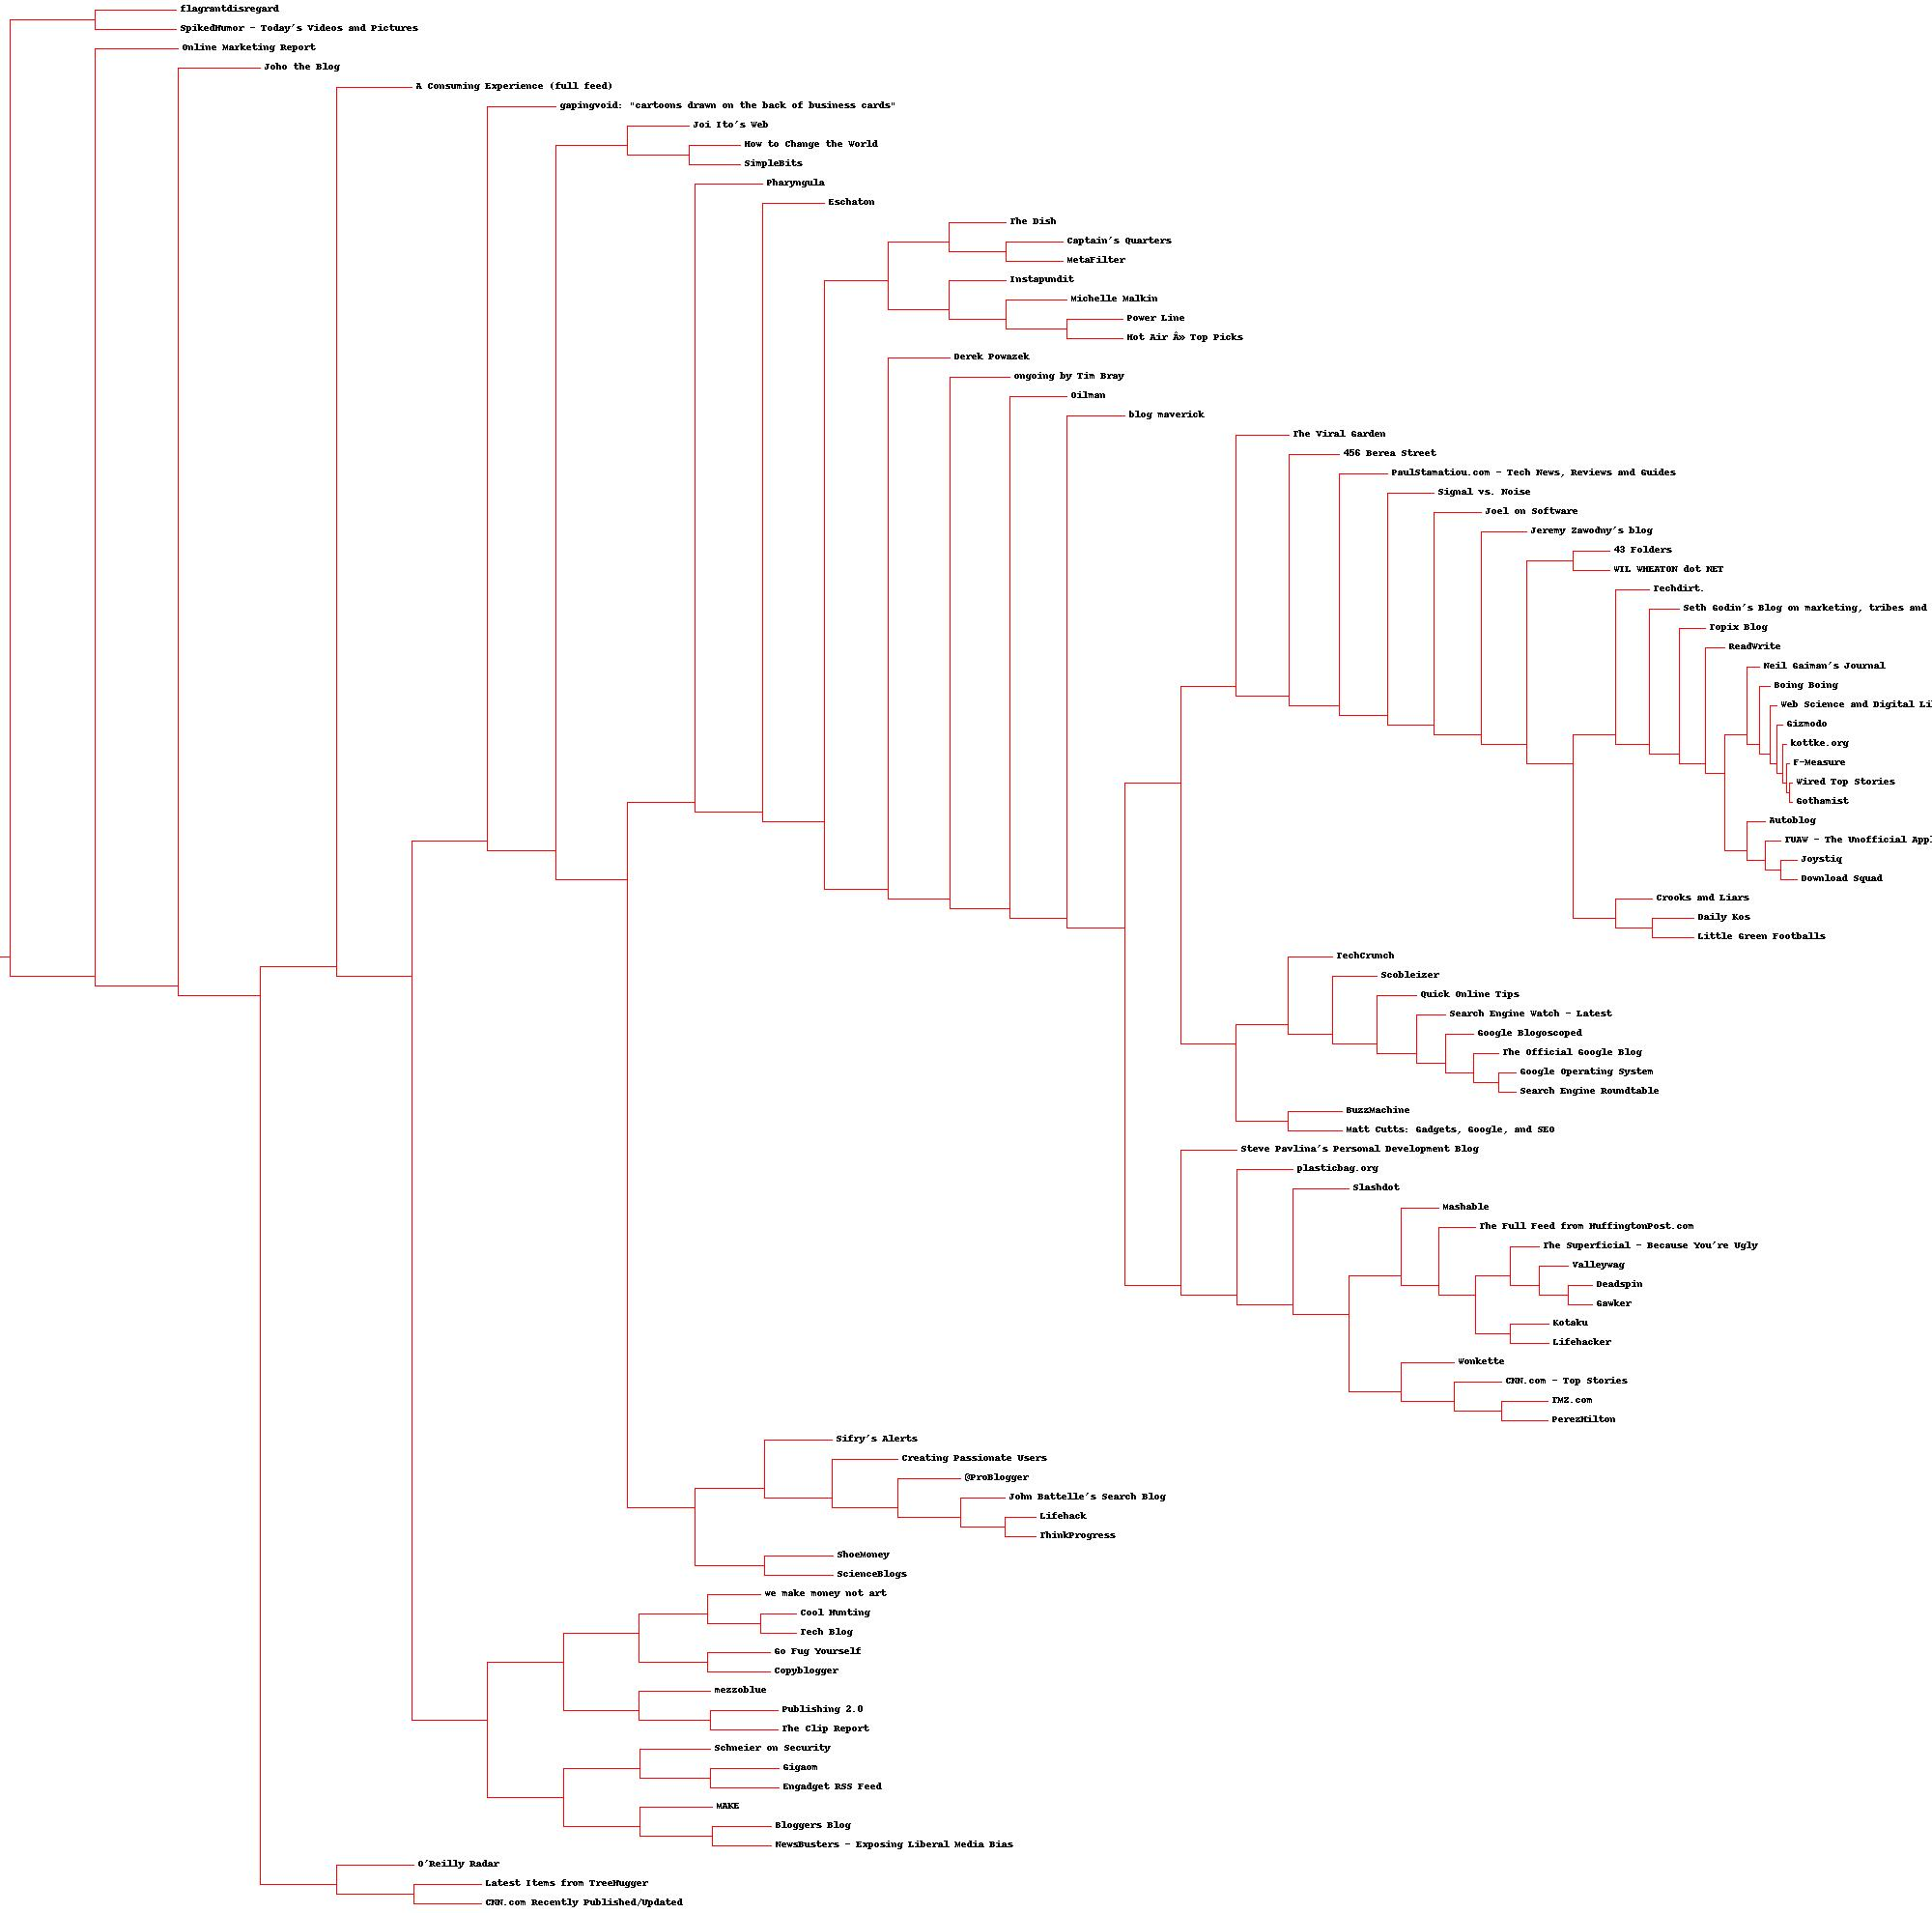
\includegraphics[width=0.8\textwidth]{Clust_Dendrogram.jpg}
\caption{Clust Dendrogram}
\label{fig:JPEG dendrogram that clusters the most similar blogs}
\end{figure}

\end{homeworkProblem}
\newpage


\clearpage

%----------------------------------------------------------------------------------------
%	PROBLEM 3
%----------------------------------------------------------------------------------------

\begin{homeworkProblem}
%Listing \ref{part3} shows a Perl script.
%\lipsum[3]

\begin{verbatim}

Cluster the blogs using K-Means, using k=5,10,20. (see slide 18).
How many interations were required for each value of k?

\end{verbatim}

\begin{verbatim}

Answer: 
Assignment9.py uses kcluster function to place a K points randomly 
in space that represent the centre of the cluster and assigns each 
blog to the nearest one. Then moves centroids to the average location 
of all the nodes that assigned to them. Repeats this process until 
the assignments stop changing.

For K = 5, there were 5 iterations needed to cluster the blogs.  
For k = 10, there were 6 iterations needed to cluster the blogs.  For 
k=20, there were 5 iterations needed to cluster the blogs. The output 
generated is found in Kinterations.txt.


\end{verbatim}
\end{homeworkProblem}
\newpage

\clearpage

%----------------------------------------------------------------------------------------
%	PROBLEM 4
%----------------------------------------------------------------------------------------

\begin{homeworkProblem}
%Listing \ref{part4} shows a Perl script.
%\lipsum[4]

\begin{verbatim}

Use MDS to create a JPEG of the blogs similar to slide 29.  
How many iterations were required?

\end{verbatim}

\begin{verbatim}

Answer: 
Assignment9.py uses 2 functions to create the MDS. Scaledown function 
takes the data vector obtained from readfile function, finds the 
difference between each pair of blogs, and matches them to a distances 
using Pearson correlation. These distances will represent the distances 
between the blogs in the chart.  Returns the X and Y coordinates of the 
blogs on the two-dimensional chart.

Function draw2d uses Python Imaging Library to to generate an image 
with all the labels of all the different blogs plotted at the 
coordinates of that blog which obtained from first function.

\end{verbatim}

\begin{figure}[!ht]
\centering
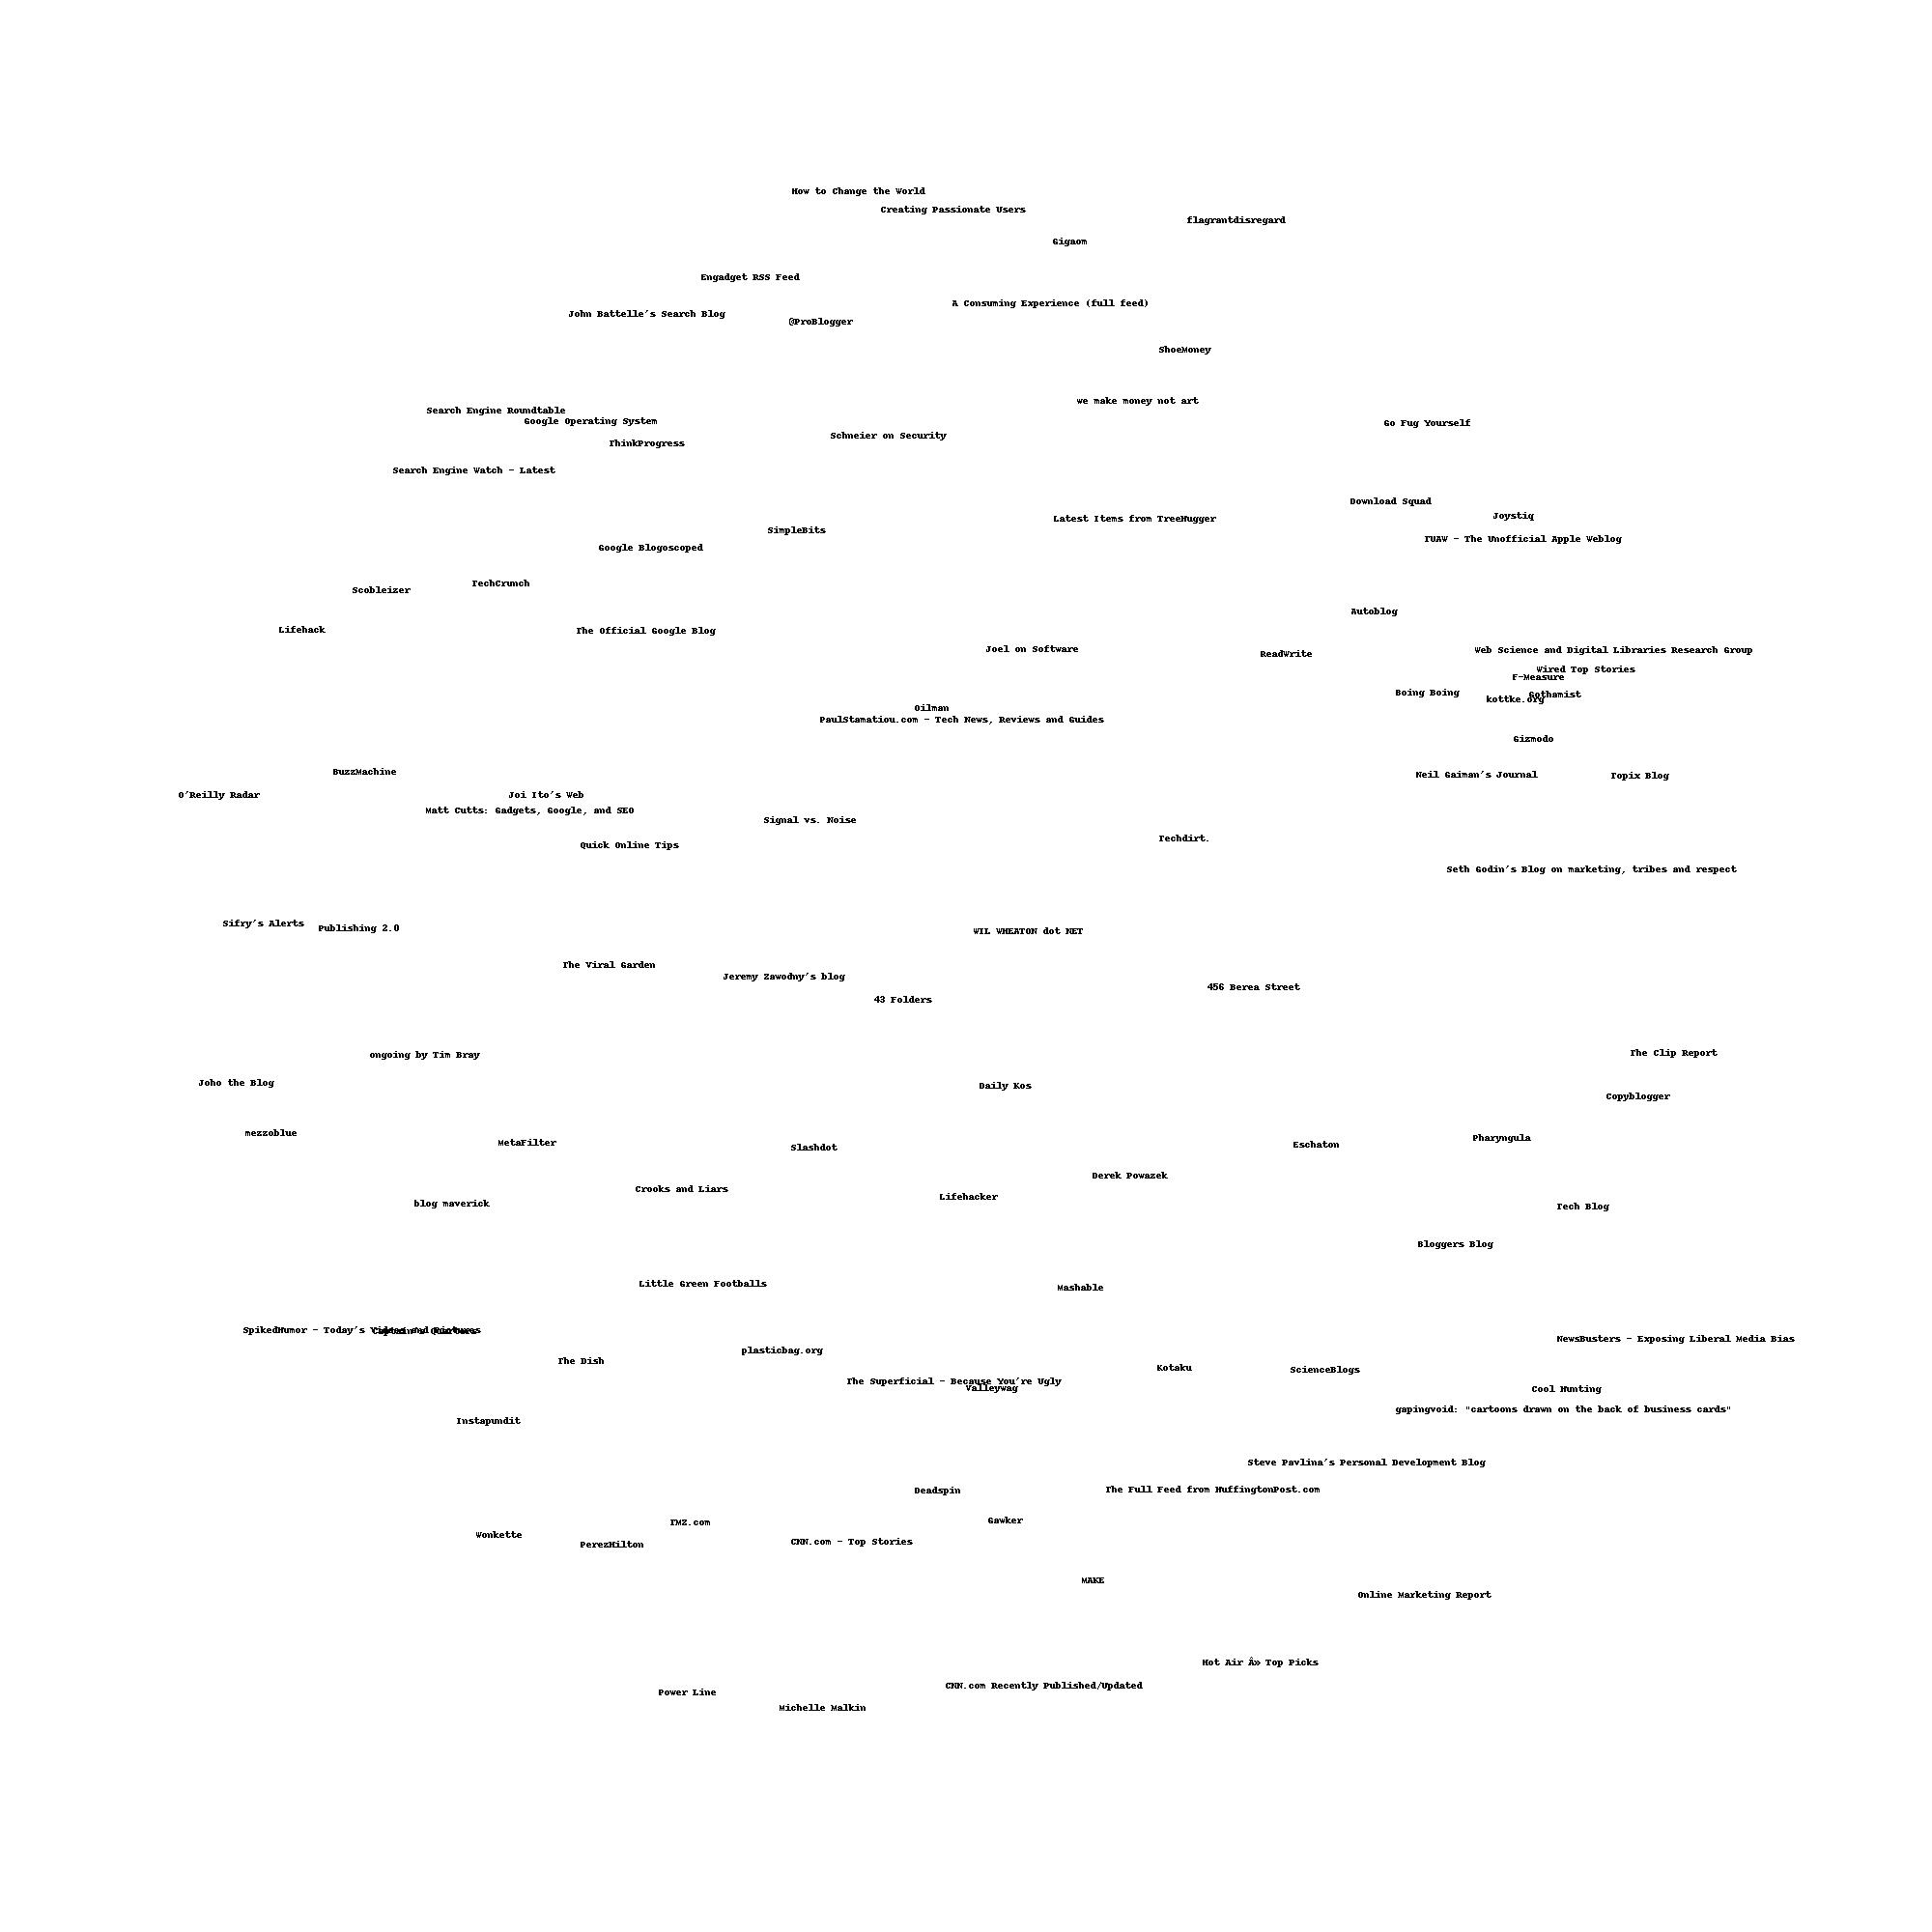
\includegraphics[width=0.8\textwidth]{MDS.jpg}
\caption{MDS}
\label{fig:MDS Blog Cloud}
\end{figure}
\newpage

\lstinputlisting[breaklines=true, caption= Assignment9 Python]{Assignment9.py}

\end{homeworkProblem}
\newpage


\clearpage
%-------------------------------------------------------------------
%References
%-------------------------------------------------------------------
\bibliographystyle{plain}
\bibliography{assignment7}


%----------------------------------------------------------------------------------------

\end{document}